%LTeX: language=it
% DOC TYPE E DEF QB SOFTWARE %%%%%%%%%%%%%%%%%%%%%%%%%
\documentclass[12pt]{article}
%%%%%%%%%%%%%%%%%%%% PACKAGES %%%%%%%%%%%%%%%%%%%%
\usepackage[english,italian]{babel}
\usepackage[a4paper, margin=3cm]{geometry}
\usepackage[T1]{fontenc}
\usepackage[utf8]{inputenc}
\usepackage[table]{xcolor}
\usepackage{amsmath}
\usepackage{graphicx}
\usepackage{float}
\usepackage{tabularx}
\usepackage{booktabs}
\usepackage{hyperref}
\usepackage{xcolor}
\usepackage{multicol}
\usepackage{multirow}
\usepackage{soul}
\usepackage{enumitem}
\usepackage{textcomp}
\usepackage{eurosym}
\usepackage{lastpage}
\usepackage{fancyhdr}
\usepackage{adjustbox}
\usepackage{subfiles}

%%%%%%%%%%%%%%%%%%%% COMMAND -> New commands %%%%%%%%%%%%%%%%%%%%
\newcommand{\mailtoQBS}
{
	\href{mailto:qbsoftware.swe@gmail.com}{qbsoftware.swe@gmail.com}
}

\let\oldpar\paragraph
\renewcommand{\paragraph}[1]{\oldpar{#1}\mbox{}\\}

%%%%%%%%%%%%%%%%%%%% COMMAND -> Redefine LaTeX Commands %%%%%%%%%%%%%%%%%%%%
\def\title#1{\gdef\THETITLE{#1}}
\def\date#1{\gdef\THEDATE{#1}}
\def\footname#1{\gdef\THEFOOTNAME{#1}}

\let\oldtexteuro\texteuro
\renewcommand{\texteuro}{\euro}

%%%%%%%%%%%%%%%%%%%% STYLES -> Commands %%%%%%%%%%%%%%%%%%%%
\newcommand{\makefirstpage}
{
	\begin{titlepage}
		
		% Defines a new command for the horizontal lines, change thickness here
		\newcommand{\HRule}{\rule{\linewidth}{0.2mm}} 
		
		\center % Center everything on the page
		
		
		%	Heading Sections
		
		\textsc{\LARGE QB Software}\\[.1cm] 
		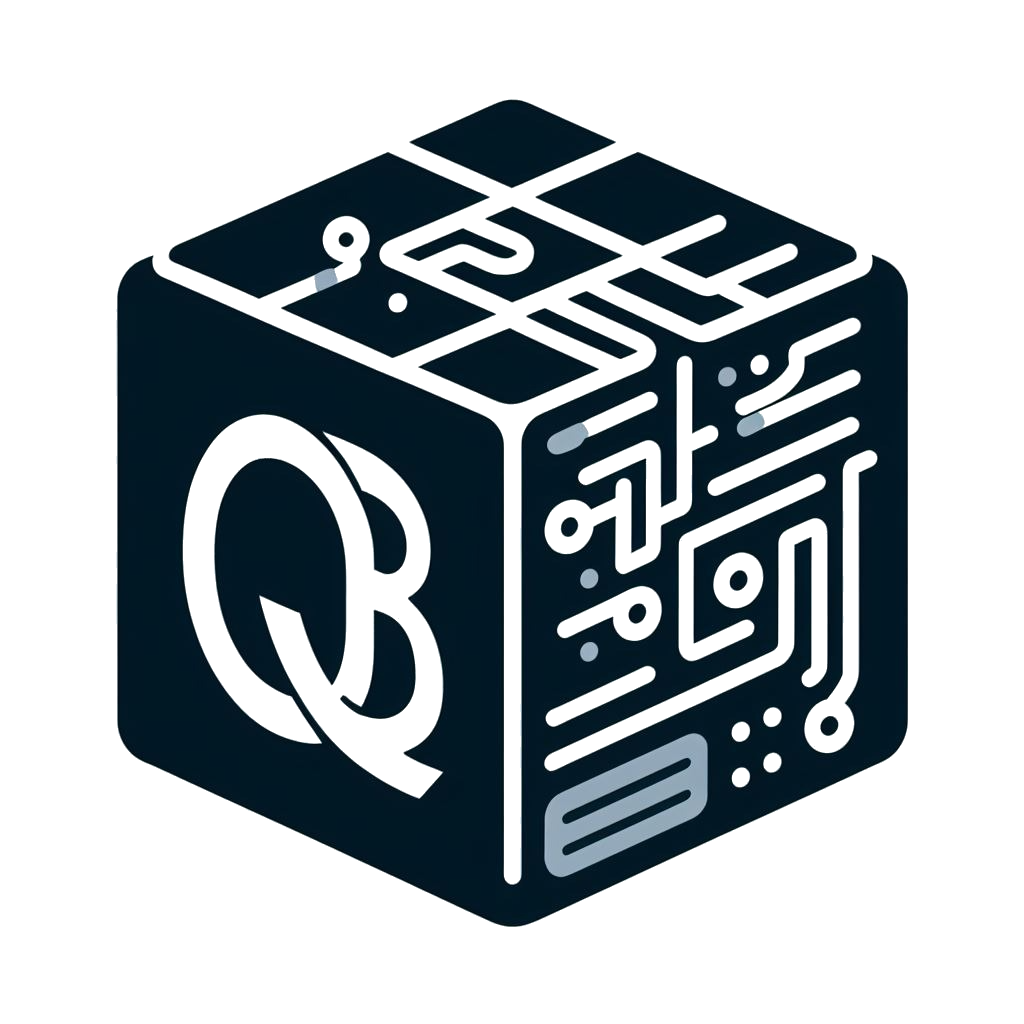
\includegraphics[scale=.15]{imgs/qb-software-logo.png}\\[-.1 cm] 
		
\includegraphics[scale=.025]{imgs/x.png}\\[0.5cm]
		
\includegraphics[scale=.3]{imgs/unipd_logo.png}\\[.5cm]
		\textsc{\Large Università degli studi di Padova}\\[0.5cm] 
		\textsc{\large corso di ingegneria del software }\\[0.5cm]
		\textsc{\large anno accademico 2023/2024 }\\[0.5cm]
		
		
		%	Title section and date section
		
		\ifdefined\THEDATE
		\HRule \\[0.4cm]
		{ \huge{ \bfseries {\THETITLE}} \\ [.5cm]
			\THEDATE}\\[0.4cm] 
		\HRule \\[0.4cm]
		\else
		\HRule \\[0.4cm]
		{ \huge{ \bfseries {\THETITLE}} } \\
		\HRule \\[0.4cm]
		\fi
		%
		\textsc{Contatti:} \mailtoQBS\\[0.3cm]
		
		\vfill 
		
	\end{titlepage}
}

%%%%%%%%%%%%%%%%%%%% ACCESSIBILITY %%%%%%%%%%%%%%%%%%%%
\let\oldhref\href
\renewcommand{\href}[2]{\oldhref{#1}{\textcolor{blue}{\ul{#2}}}}

\hypersetup{
	colorlinks = true,
	linkcolor = cyan,
}

%%%%%%%%%%%%%%%%%%%% STYLES -> Settings %%%%%%%%%%%%%%%%%%%%
% Enable header and footer style
\pagestyle{fancy}
\thispagestyle{empty}
\thispagestyle{fancy}
\pagestyle{fancy}

% Header
\setlength{\topmargin}{-40pt}
\setlength{\headsep}{60pt}
\fancyhf{}
\lhead{QB Software}
\setlength{\headheight}{15pt}
\rhead{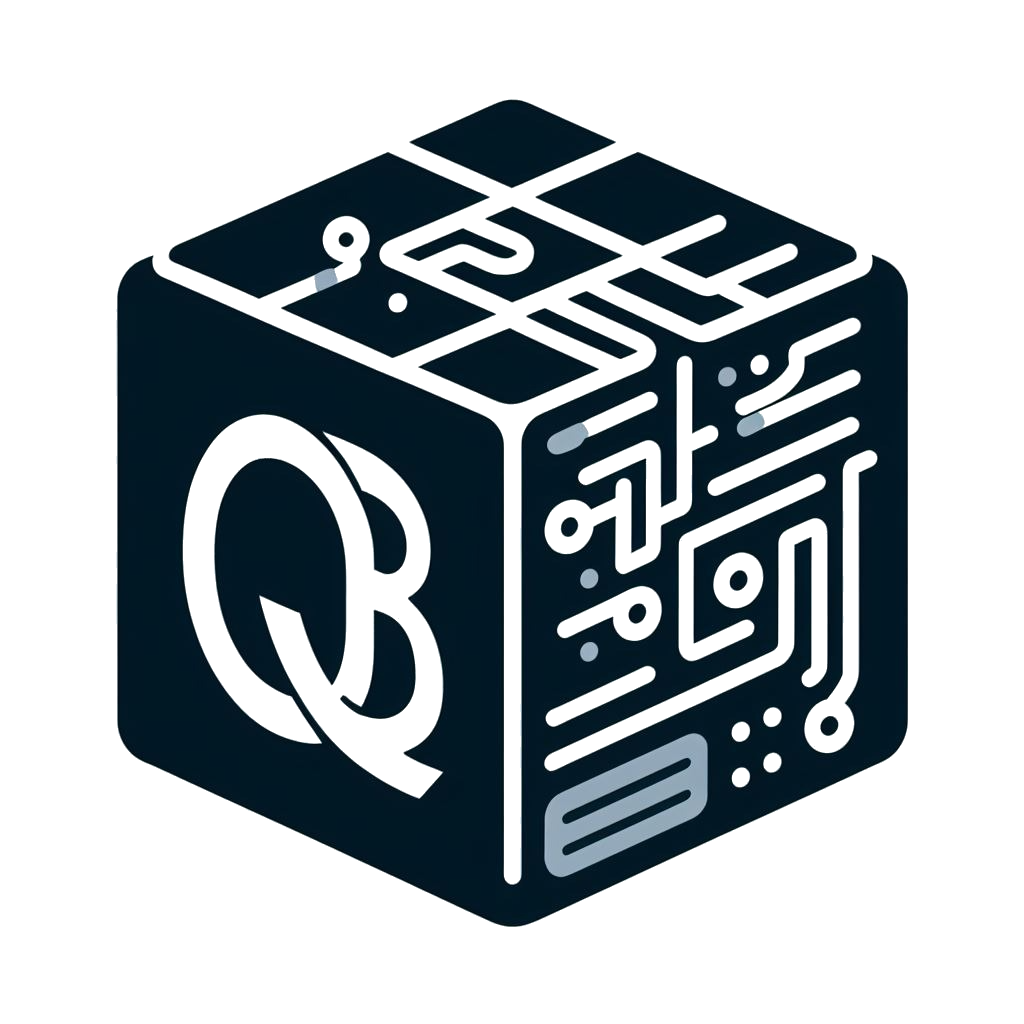
\includegraphics[width=1cm]{imgs/qb-software-logo.png}}

% Footer 
\fancyfoot{}
\fancyfoot[L]{\THEFOOTNAME}
\fancyfoot[R]{Pagina \thepage~di~\pageref{LastPage}}
\futurelet\TMPfootrule\def\footrule{\TMPfootrule}
\setcounter{page}{0}
\pagenumbering{arabic}
\renewcommand{\footrulewidth}{0.3pt}

%%%%%%%%%%%%%%%%%%%% ENVIRONMENT %%%%%%%%%%%%%%%%%%%%
% Remove colorless padding in booktabs
\setlength{\aboverulesep}{0cm}
\setlength{\belowrulesep}{0cm}
\setlength{\extrarowheight}{.75ex}

\newenvironment{todo}{
	\rowcolors{2}{cyan!80!black!30!}{cyan!80!black!20!}
	\begin{tabular}{p{3.48cm}>{\raggedright\arraybackslash}p{4cm}>{\raggedright\arraybackslash}p{6.5cm}}
		\toprule
		\rowcolor{gray!20} \textbf{ID}	& \textbf{Interessato} & \textbf{Task} 
		\\\midrule
	}{
		\bottomrule
	\end{tabular}
}

\newenvironment{changelog}{
	\noindent
	{\Large \textbf{Registro delle modifiche}}
	\noindent
	\begin{table}[h]
		\rowcolors{2}{cyan!80!black!30!}{cyan!80!black!20!}
		\begin{adjustbox}{width=\textwidth}
			\begin{tabular}{|c|c|p{2.35cm}|c|p{3.3cm}|}
				\hline
				\rowcolor{gray!20}
				\textbf{V.} & \textbf{Data} & \textbf{Membro} & \textbf{Ruolo} & \textbf{Descrizione} \\
				
				\hline
			}{
				\hline
			\end{tabular}
		\end{adjustbox}
	\end{table}
	
	\clearpage
}

% 1   2    3        4             5            6            7          
% Ver Data Relatore RuoloRelatore DataVerifica Verificatore Descrizione
\newcommand{\newlog}[7]{
	#1 & #5 & #6 & Verificatore & Controllo qualità \\
	   & #2 & #3 & #4           & #7 \\\hline
}

% INFORMAZIONI DOCUMENTO %%%%%%%%%%%%%%%%%%%%%%%%%
\title{Verbale esterno}
\date{del 11/12/2023}
\footname{Verbale esterno del 11/12/2023}

\begin{document}
	% PRIME PAGINE %%%%%%%%%%%%%%%%%%%%%%%%%
	\makefirstpage
	
	% 1   2    3        4             5            6            7          
% Ver Data Relatore RuoloRelatore DataVerifica Verificatore Descrizione
\begin{changelog}
	\newlog{0.3.0}{15/12/2023}{S. Rovea}{Amministratore}{/12/2023}{}{Correzione ed espansione sezione \ref{sec:management_process}}
	\newlog{0.2.0}{02/12/2023}{S. Destro}{Amministratore}{03/12/2023}{A. Feltrin}{Aggiunta sezione su processi organizzativi, sezione \ref{sec:management_process}}
	\newlog{0.1.0}{22/11/2023}{A. Bustreo}{Amministratore}{22/11/2023}{A. Giurisato}{Aggiunto processo supporto per la documentazione, sezione \ref{sec:documentation}. Aggiunta prefazione, sezione \ref{sec:prefazione}}
\end{changelog}
	\clearpage
	
	\tableofcontents
	\clearpage

    \section{Informazioni generali}
    
    \subsection{Luogo e data dell'incontro}
    
    \begin{itemize}
    	\item \textbf{Luogo}: meeting su Zextras Chat
    	\item \textbf{Data}: 11/12/2023
    	\item \textbf{Ora di inizio}: 15:15
    	\item \textbf{Ora di fine}: 16:00
    \end{itemize}
    
    \subsection{Presenze}
    
    \begin{itemize}
    	\item \textbf{Totale presenze}:
    	\begin{itemize}
    		\item Bustreo Alessandro
    		\item Destro Stefano
    		\item Domuta Alessia 
    		\item Feltrin Alessandro 
    		\item Fontana Raffaele Paolo 
    		\item Giurisato Andrea 
    		\item Rovea Silvia
    	\end{itemize}
    	
    	\item \textbf{Totale assenze}: 0
    	
    	\item \textbf{Partecipanti esterni}:
    	\begin{itemize}
    		\item Federico Rispo (Zextras)
    	\end{itemize}
    \end{itemize}
    
    \section{Ordine del giorno}
    \begin{itemize}
    	\item Domande da porre all'azienda.
    \end{itemize}
    
    \section{Verbale}
    Le domande poste da QB Software a Zextras durante il meeting:

    \newcommand{\answer}{\item[\textbf{A:}]}
        
        \begin{enumerate}[label=\textbf{Q\arabic*:}]
            \item In vista delle vacanze, per quale periodo dobbiamo sospendere i meeting con voi?
            \answer Dal 25 dicembre fino al 7 gennaio.

            \item Per testare lo scambio di e-mail tra server dobbiamo usare dei domini? E se sì, potete metterci a disposizione dei domini su cui sperimentare? 
            \answer Non è necessario, potete sviluppare tutto in locale.

            \item Dobbiamo implementare tutto il sistema di scambio dell'e-mail? Quindi, implementare la comunicazione attraverso SMTP tra il prodotto che dobbiamo sviluppare e altri server sulla rete?
            \answer L'e-mail non deve essere inviata a un provider esterno, si dà per scontato che la email viene inviata e ricevuta dal sistema esterno. L'obiettivo è implementare il protocollo JMAP, quindi non è obbligatorio implementare il SMTP.
            
            \item Stiamo affrontando dei problemi con Java 21, possiamo utilizzare un'altra versione LTS? 
            \answer Certo, usate Java 17.
        
            \item È consigliato usare Guice per la dependency injection?
            \answer Guice è consigliato, ma non è obbligatorio.
        \end{enumerate}

        \noindent
        Il proponente ci ha consigliato di valutare le tecnologie Hikari e Quarkus, perché potrebbero essere utili nel progetto. Nell'ultima parte della riunione c'è stato una discussione sull'utilità di utilizzare MongoDB al posto di Postgre, visto che JMAP basa l'intero protocollo sull'uso del formato JSON.
    
    \section{Azioni da intraprendere}
    Proseguire con lo studio delle tecnologie.
\end{document}